\section{Introduction}
\label{sec:intro}
Local distance-ladder measurements of the Hubble constant $H_0$ disagree with the value inferred from the cosmic microwave background in flat $\Lambda$CDM \citep{riess2022shoes,planck2020cosmology}. Methods with independent systematics are therefore valuable. Two of them are standard sirens, in which the amplitude of a compact-binary gravitational wave (GW) gives the luminosity distance \citep{schutz1986,holz2005,lvk2017h0}, and time-delay cosmography, in which the delays between the images of a strongly lensed source give the time-delay distance \citep{refsdal1964,treu2016review,wong2020h0licow,birrer2020tdcosmo,tdcosmo2025}. Time-delay cosmography with lensed quasars is limited by the lens mass model. At fixed image positions the predicted delay scales with the radial slope of the lens profile \citep{wucknitz2002,kochanek2002}, and an external mass sheet rescales all delays without changing the image positions or the magnification ratios (the mass-sheet degeneracy) \citep{falco1985msd,schneider2013msd}.

Strongly lensed binary black holes (BBHs) are expected at a rate of order one per year at the sensitivity of the next LIGO--Virgo--KAGRA observing runs and in much larger numbers with the Einstein Telescope (ET) \citep{ng2018rates,li2018statistical,oguri2018distribution,wierda2021beyond}; none has yet been confirmed \citep{lvk2021o3a,lvk2024o3search,lvk2025gwtc4lensing}. If the host galaxy and the lens are identified, such a system combines the two methods. Liao et al.~\citep{liao2017precision} proposed this measurement, combining the delays of lensed GW signals with the images and redshifts observed in the EM domain, and forecast that ten such systems detected by ET would constrain $H_0$ to 0.7\% in flat $\Lambda$CDM, assuming uncertainties of 0.6\% in the Fermat-potential difference predicted by the lens model and of 1\% from the line of sight (see also Refs.~\citep{fan2017speed,hannuksela2020localizing}). The delay is measured to milliseconds, so it has no measurement error that matters for cosmography and no uncertainty from source variability or microlensing of an extended source. The amplitude of each image gives its apparent distance $d_L/\sqrt{|\mu|}$, where $\mu$ is the magnification, so that an absolute magnification predicted by the lens model can be compared with the GW data. Imaging of the lensed host constrains the lens model \citep{hannuksela2020localizing,wempe2022lensing,uronen2026silmarel,uronen2026galacticcentres}, and spectroscopy gives the lens and source redshifts. The mass-sheet degeneracy is not broken by these data: the GW apparent distance and the delay both scale with the mass sheet in the same way as with $1/H_0$ \citep{poon2025degeneracy}. Without a host, lensed GWs constrain cosmology only statistically \citep{jana2023cosmography}.

Such forecasts take the uncertainty of the lens model as given and assume that the analysis is unbiased. Whether a population of such systems gives an unbiased $H_0$ when the GW data and the lens are analyzed in full has not been tested. Unbiased inference requires that the priors of the analysis describe the population that produced the observed systems, and that the selection of the systems be accounted for. Both conditions are known to matter for lensed quasars, whose selection favors lenses with shallow density profiles \citep{collett2016selection,li2024selection}. For lensed GWs, selection is on the signal-to-noise ratio (SNR), which at fixed redshift depends on $H_0$ itself.

In this paper we perform this test on simulated systems. We use the lensed BBHs of a companion paper \citep{paper1} (hereafter Paper~I), which benchmarks how well the absolute magnification of such systems can be measured. For 60 systems detected by ET and 59 detected by an O5-like network, we infer $H_0$ from the GW data, obtained by joint parameter estimation of both images from simulated detector data, together with a Bayesian reconstruction of the lens from the electromagnetic (EM) data. We show that two corrections are required for an unbiased result, measure the precision per system and for the combined sample, and identify where the information on $H_0$ comes from. Section~\ref{sec:principle} sets out the observables and their degeneracies, Sec.~\ref{sec:systems} the simulated systems, Sec.~\ref{sec:inference} the inference, including a worked example, Sec.~\ref{sec:results} the results, and Sec.~\ref{sec:discussion} what they imply for real data. Appendix~\ref{app:example} gives the posteriors of all parameters of the worked example, Appendix~\ref{app:calibration} checks the calibration of the per-system posteriors, and Appendix~\ref{app:full} the approximation of the GW likelihood against full sampling of the strain data together with the lens model.

\section{The Hubble constant from a lensed GW with an identified host}
\label{sec:principle}
\subsection{Observables}
\label{sec:observables}
Figure~\ref{fig:schematic}(a) shows the configuration. A BBH merges in a host galaxy at redshift $z_s$; a galaxy at $z_l$ along the line of sight produces two or more images, of which $A$ and $B$ denote the two GW images (the pair of images detected in the GW data, $A$ having the larger measured SNR). The GW data give three lensing observables. The arrival-time difference $\Delta t=t_B-t_A$ is measured to milliseconds. The amplitude of image $j$ is that of an unlensed source at the apparent distance $D_j=d_L/\sqrt{|\mu_j|}$, where $d_L$ is the luminosity distance of the source and $\mu_j$ the magnification, so the two amplitudes give the magnification ratio $\mu_B/\mu_A$ and, with the chirp mass and inclination, the apparent distance $D_A$. The Morse index $n_j$ of each image ($0$, $\frac12$ or $1$ for an image at a minimum, saddle point or maximum of the arrival-time surface) shifts the phase of the waveform by $-n_j\pi$ and is partly measurable when the waveform contains higher harmonics \citep{dai2017morse,janquart2023golum,lo2023bayesian}. The EM data give the positions $\boldsymbol\theta_A$, $\boldsymbol\theta_B$ of the images relative to the center of the lens light, the shape of the lens light, the velocity dispersion $\sigma_v$ of the lens and the spectroscopic redshifts $z_l$ and $z_s$.

A lens model with parameters $\boldsymbol\eta$ and a source position $\boldsymbol\beta$ predict the image positions, the magnifications $\mu_A$, $\mu_B$, the Morse indices and the difference $\Delta\phi$ of the Fermat potentials of the two images, all in angular units. The dimensional observables follow from the distances. We allow for an external convergence $\kappa_{\rm ext}$, a uniform mass sheet from structures along the line of sight, and write $h\equiv H_0/H_0^{\rm true}$. In flat $\Lambda$CDM with fixed matter density all distances at fixed redshift scale as $1/h$, and
\begin{align}
\Delta t&=(1-\kappa_{\rm ext})\,\frac{D_{\Delta t}(z_l,z_s)}{h\,c}\,\Delta\phi,\label{eq:dt}\\
D_A&=\frac{d_L(z_s)}{\sqrt{|\mu_A|}}=(1-\kappa_{\rm ext})\,\frac{d_L(z_s)}{h\,\sqrt{|\mu_A^{(0)}|}},\label{eq:da}
\end{align}
where $D_{\Delta t}=(1+z_l)D_lD_s/D_{ls}$ is the time-delay distance and $d_L$ the luminosity distance of the true cosmology ($D_l$, $D_s$ and $D_{ls}$ are angular-diameter distances to the lens, to the source and between them), and $\mu^{(0)}$ is the magnification without the sheet, so that $\mu=\mu^{(0)}/(1-\kappa_{\rm ext})^2$. The image positions and the magnification ratio do not depend on $\kappa_{\rm ext}$ or $h$. The velocity dispersion sets the Einstein radius through the ratio $D_{ls}/D_s$, which does not depend on $h$ either; it fixes the mass normalization without a distance scale. The delay therefore measures $h$ through Eq.~\eqref{eq:dt} once the lens model fixes $\Delta\phi$, and the apparent distance tests the absolute magnification of the same model through Eq.~\eqref{eq:da}.

\begin{figure*}
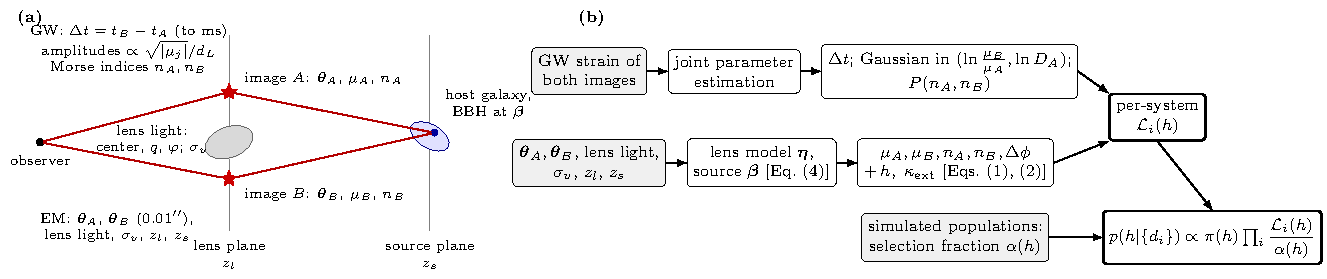
\includegraphics[width=\textwidth]{fig_schematic.pdf}
\caption{(a) A lensed BBH with an identified host. The GW data of the two images $A$ and $B$ give the delay $\Delta t$, the amplitudes, which depend on the magnifications $\mu_j$ and the luminosity distance $d_L$, and the Morse indices $n_j$; the EM data give the image positions relative to the lens light, the shape of the lens light, the velocity dispersion $\sigma_v$ and the redshifts. (b) The inference of this paper. Joint parameter estimation of both GW images is summarized as an effective likelihood (Sec.~\ref{sec:gwlike}); a lens model with the priors of Table~\ref{tab:priors} and the normalized source-position prior predicts the GW observables through Eqs.~\eqref{eq:dt} and \eqref{eq:da}; the per-system likelihoods $\mathcal L_i(h)$ are combined with the selection fraction $\alpha(h)$ by Eq.~\eqref{eq:joint}.}
\label{fig:schematic}
\end{figure*}

\subsection{Degeneracies}
\label{sec:degeneracies}
Both observables depend on $(1-\kappa_{\rm ext})/h$ only, so $h$ and $\kappa_{\rm ext}$ are exactly degenerate \citep{poon2025degeneracy}: the mass-sheet degeneracy of time-delay cosmography is not broken by the GW amplitudes. A prior on $\kappa_{\rm ext}$ therefore sets a floor on the uncertainty of $h$ for each system, and an error in its mean biases $h$ by the same amount for every system.

The second degeneracy is with the radial slope of the lens. At fixed image positions, a steeper lens profile predicts a longer delay: the delay depends on the mean convergence between the images \citep{kochanek2002}, and for a power-law lens with three-dimensional density $\rho\propto r^{-\gamma'}$ ($\gamma'=2$ isothermal) the Fermat-potential difference of two images at fixed positions is proportional to $\gamma'-1$ to first order around $\gamma'=2$ (see also \citep{wucknitz2002}). At a measured delay, therefore,
\begin{equation}
\delta\ln h\simeq\frac{\delta\gamma'}{\gamma'-1}\approx\delta\gamma'\quad(\gamma'\approx2).
\label{eq:slope}
\end{equation}
An error of 0.05 in the slope is a 5\% error in $H_0$. Two image positions and a magnification ratio constrain the slope only weakly, so the prior on $\gamma'$ matters. The slope is also the main source of error of the magnification (Paper~I), which is why the GW apparent distance, Eq.~\eqref{eq:da}, could in principle constrain $H_0$ beyond the delay. We quantify this in Sec.~\ref{sec:information}.

\section{Simulated systems}
\label{sec:systems}
\subsection{Populations, detection and the analyzed sample}
\label{sec:populations}
The lensed BBHs are those of the joint parameter-estimation tests of Paper~I: 15 systems for each of four lens families and each of two detector scenarios, drawn at random from simulated catalogs of detected systems. The lens families are the singular isothermal sphere (SIS), the singular isothermal ellipsoid (SIE), the SIE with external shear, and the elliptical power law (EPL) with external shear, whose slope $\gamma'$ is drawn from $\mathcal N(2.08,0.15)$ \citep{auger2010slacs,tessore2015epl}. The detector scenarios are the ET-D design \citep{hild2011etd} and an O5-like network of the two LIGO detectors at A+ and Virgo at design sensitivity. Sources follow the GWTC-4.0 BBH population \citep{lvk2025gwtc4pop} and a merger rate that traces the star-formation history, weighted by the lensing optical depth; lens redshifts and velocity dispersions follow the isothermal lensing statistics. The source is placed uniformly within the region of the source plane in which the lens produces at least two images (the multiple-image region). A system is detected if two images have a network SNR $\hat\rho=\rho+\mathcal N(0,1)\ge8$ within one year and the two GW images are separated by at least 0.1\,arcsec. All distances are computed in the Planck18 cosmology \citep{planck2020cosmology}, so that the true value is $h=1$. One O5 system whose catalog entry cannot be reproduced from the stored inputs is excluded, as in Paper~I, leaving 60 ET and 59 O5 systems.

\begin{figure*}
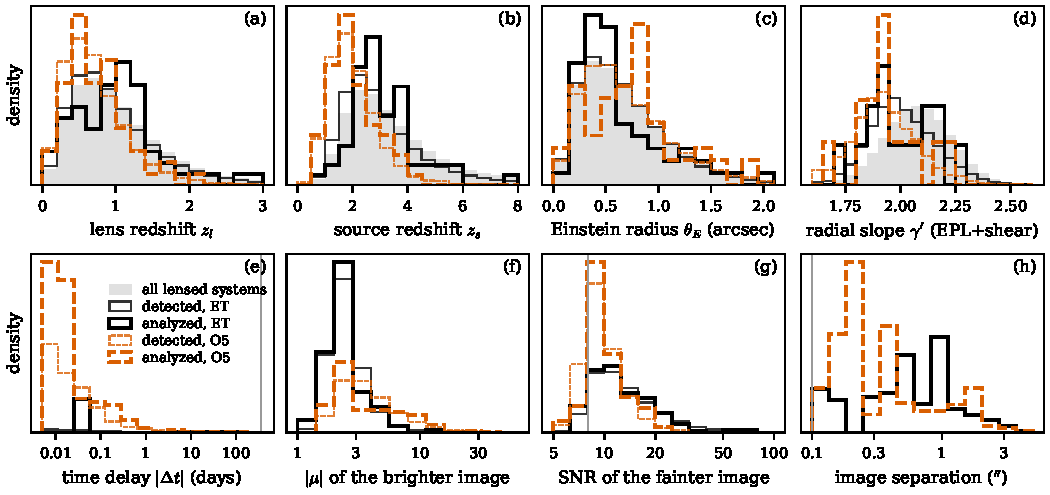
\includegraphics[width=\textwidth]{fig_sample.pdf}
\caption{The analyzed systems (thick histograms: 60 ET, solid; 59 O5, dashed) against the simulated populations: all lensed systems of the catalogs (gray) and those passing the detection criteria (thin lines), with the four lens families weighted equally. (a)--(d) Lens redshift, source redshift, Einstein radius and, for the EPL+shear family, the radial slope. (e)--(h) Time delay, magnification of the brighter GW image, network SNR of the fainter image and separation of the two GW images, which are defined for detected systems only. Vertical lines: the one-year window, the SNR threshold of 8 (the detection statistic adds unit noise to the SNR shown) and the 0.1-arcsec separation cut.}
\label{fig:sample}
\end{figure*}

Figure~\ref{fig:sample} and Table~\ref{tab:sample} describe the analyzed systems against the populations they come from. ET detects 42--51\% of all lensed systems, depending on the family, and its detected systems resemble the parent population: typical source redshifts of 3, Einstein radii of 0.5\,arcsec, delays of 50\,days and magnifications of the brighter image of 2--3; only 11--14\% have a magnification above 5 and fewer than 7\% are four-image systems. O5 detects about 1\%, and these are the most magnified systems: half have a magnification above 5, a third are four-image systems whose GW images are the merging pair near a fold caustic, and the median delay is 11--18\,days. The analyzed samples follow the detected populations within their sampling fluctuations. The slope distribution of the detected EPL+shear lenses is shifted below the parent distribution, to a mean of 2.01 for ET and 1.93 for O5 against 2.08 [Fig.~\ref{fig:sample}(d)], because shallower profiles produce larger magnifications; this selection effect is known from lensed quasars \citep{collett2016selection,li2024selection} and matters for the choice of prior (Sec.~\ref{sec:selection}).

\begin{table}
\caption{The analyzed systems: median and 10--90\% range of the true quantities, and numbers of systems. Image $A$ is the GW image with the larger measured SNR.}
\label{tab:sample}
\footnotesize
\begin{tabular*}{\linewidth}{@{\extracolsep{\fill}}lcc@{}}
\toprule
 & ET (60 systems) & O5 (59 systems)\\
\midrule
Lens redshift $z_l$ & 0.99 (0.30--1.68) & 0.67 (0.23--1.21)\\
Source redshift $z_s$ & 2.89 (1.85--4.88) & 1.90 (1.02--3.21)\\
Einstein radius $\theta_E$ (arcsec) & 0.48 (0.24--1.31) & 0.74 (0.24--1.39)\\
Image separation (arcsec) & 0.99 (0.43--2.63) & 1.10 (0.21--2.18)\\
Time delay $|\Delta t|$ (days) & 47.1 (8.2--172.2) & 11.3 (0.1--78.1)\\
$|\mu|$ of the brighter image & 2.6 (1.9--5.0) & 6.2 (2.3--15.7)\\
Network SNR, image $A$ & 27.4 (16.5--61.9) & 14.6 (9.9--22.2)\\
Network SNR, image $B$ & 13.8 (8.7--31.7) & 10.2 (8.2--17.8)\\
Four-image systems & 2 & 22\\
Systems with $|\mu|\ge5$ & 6 & 37\\
Image $A$ at a saddle point & 11 & 16\\
\bottomrule
\end{tabular*}

\end{table}

\subsection{GW data}
\label{sec:gwdata}
For each system both images were injected into stationary Gaussian noise with the \textsc{IMRPhenomXHM} waveform, which includes higher harmonics \citep{garciaquiros2020xhm}, and analyzed jointly with \textsc{bilby} \citep{ashton2019bilby}, the \textsc{dynesty} nested sampler \citep{speagle2020dynesty} and relative binning \citep{zackay2018relbin,krishna2023relbin} (Paper~I). The joint analysis samples the source parameters shared by both images and, for the lensing, the magnification ratio $\mu_B/\mu_A$, the apparent distance $D_A$, the delay $\Delta t$ and the Morse index of each image. For ET the sky position is fixed to that of the identified host, because a single ET site constrains it poorly; for O5 it is free.

\subsection{EM data}
\label{sec:emdata}
The EM data of each system are the positions of the images relative to the center of the lens light, measured to 0.01\,arcsec, the light center itself (0.02\,arcsec), the axis ratio and position angle of the lens light (which trace those of the mass with scatter 0.05 and $10\degr$), the velocity dispersion of the lens (10\%) and spectroscopic redshifts of lens and source. The positions of the BBH images within the host are assumed to have been reconstructed to the stated precision from imaging of the lensed host \citep{hannuksela2020localizing,wempe2022lensing,uronen2026silmarel}; this is an upstream step that we do not simulate (Sec.~\ref{sec:limitations}).

\section{Inference}
\label{sec:inference}
Figure~\ref{fig:schematic}(b) summarizes the analysis. Each system is analyzed in two stages: the joint parameter-estimation posterior of the GW data is summarized as an effective likelihood for the quantities that a lens model predicts (Sec.~\ref{sec:gwlike}), and the lens parameters, the source position, $\kappa_{\rm ext}$ and $h$ are then sampled with this likelihood and the EM likelihood (Sec.~\ref{sec:lensmodel}). Two ingredients are needed for the combination of systems to be unbiased: the source-position prior must be normalized for each lens model (Sec.~\ref{sec:sourceprior}), and the likelihood of each system must be divided by the fraction of systems that would be detected at the assumed $h$ (Sec.~\ref{sec:selection}). Section~\ref{sec:example} works through one system.

\subsection{GW likelihood}
\label{sec:gwlike}
The posterior of $(\ln\mu_B/\mu_A,\ln D_A)$ from the joint analysis, divided by its priors (uniform in $\ln\mu_B/\mu_A$ and $\propto D_A^2$), is approximated by a two-dimensional Gaussian, and the Morse indices enter through their posterior probabilities $P(n_A,n_B)$ (Paper~I, Appendix~C). The delay is fixed at its posterior median, because its uncertainty of milliseconds is negligible compared with the delays of days to months. Appendix~\ref{app:full} compares this two-stage approach with sampling the strain data of both images together with the lens model.

\subsection{Lens model, priors and the Hubble constant}
\label{sec:lensmodel}
Each system is analyzed with a lens model of its own family (the simulated family) or with an EPL+shear model for every system. The parameters are the velocity dispersion, which sets the Einstein radius through the isothermal relation at the observed redshifts, the lens center, the axis ratio $q$ and orientation, the external-shear strength $\gamma_{\rm ext}$ and orientation, and the slope $\gamma'$, as appropriate for the model. Table~\ref{tab:priors} lists their priors, which are the distributions of the simulated population, and the EM measurements that enter the likelihood. The image-position likelihood marginalizes over the source position with the prior of Sec.~\ref{sec:sourceprior}; the lens-light and velocity-dispersion terms are those of Paper~I (Appendix~C). The velocity dispersion is not interpreted with a dynamical model and does not constrain the mass sheet.

\begin{table}
\caption{Parameters of the lens analysis and their priors, which are the distributions of the simulated population, and the EM measurements of the likelihood. The orientations of the mass and of the light are related through the light--mass misalignment of $10\degr$. $\mathcal N(m,s)$ denotes a Gaussian of mean $m$ and standard deviation $s$, truncated to the stated range.}
\label{tab:priors}
\footnotesize
\begin{tabularx}{\linewidth}{@{}lL@{}}
\toprule
Parameter & Prior \\
\midrule
Velocity dispersion $\sigma_v$ & velocity-dispersion function weighted by $\sigma_v^4$, 100--400\,km\,s$^{-1}$ \\
Lens center & $\mathcal N(0,0.02'')$ per axis about the light center \\
Axis ratio $q$ (SIE, EPL) & $\mathcal N(0.75,0.15)$ on $[0.35,0.99]$ \\
Orientation (SIE, EPL) & uniform \\
Shear $\gamma_{\rm ext}$ (with shear) & $\ln\gamma_{\rm ext}\sim\mathcal N(\ln0.05,0.6)$ on $[10^{-3},0.25]$ \\
Shear orientation & uniform \\
Slope $\gamma'$ (EPL+shear) & $\mathcal N(2.08,0.15)$ on $[1.6,2.6]$ \\
Source position $\boldsymbol\beta$ & Eq.~\eqref{eq:sourceprior}, within the multiple-image region \\
External convergence $\kappa_{\rm ext}$ & $\mathcal N(0,0.025)$, at the value fixed by Eq.~\eqref{eq:dt} \\
$h=H_0/H_0^{\rm true}$ & uniform on $[0.5,1.5]$ \\
\midrule
Measurement & Uncertainty \\
\midrule
Image positions & 0.01\,arcsec per axis \\
Lens-light axis ratio, orientation & 0.05, $10\degr$ \\
Velocity dispersion & 10\% \\
Redshifts $z_l$, $z_s$ & spectroscopic \\
\bottomrule
\end{tabularx}
\end{table}

For each lens model and $h$, Eq.~\eqref{eq:dt} with the measured delay fixes $1-\kappa_{\rm ext}$, and the prior of $\kappa_{\rm ext}$, $\mathcal N(0,0.025)$, typical of line-of-sight estimates for lensed quasars \citep{rusu2017kext}, is evaluated there, including the Jacobian $|{\rm d}\kappa_{\rm ext}/{\rm d}\Delta t|$. The magnifications and the apparent distance then follow from Eq.~\eqref{eq:da} and are compared with the GW likelihood. The prior of $h$ is uniform in $[0.5,1.5]$. We sample the posterior of $h$ and the lens parameters with \textsc{dynesty} (500 live points) and \textsc{lenstronomy} \citep{birrer2018lenstronomy,birrer2021lenstronomy}.

\subsection{First correction: the source-position prior}
\label{sec:sourceprior}
The image-position likelihood depends on the unobserved source position $\boldsymbol\beta$, which is marginalized over. A uniform prior in $\boldsymbol\beta$ with the same normalization for every lens model is the natural choice, but it does not describe the simulated population. There, a lens is drawn from the population and the source is then placed uniformly within its multiple-image region, of area $A_{\rm mult}$; the source density is $1/A_{\rm mult}$ for that lens. The simulation draws the source within a disk of radius $R\theta_E$ and redraws it, up to 60 times, until it is multiply imaged; if a fraction $a$ of the disk lies in the multiple-image region, $A_{\rm mult}=a\,\pi(R\theta_E)^2$ and the lens is retained with probability $1-(1-a)^{60}$. The prior consistent with the population is therefore
\begin{equation}
p(\boldsymbol\beta|\boldsymbol\eta)=\frac{1-[1-a(\boldsymbol\eta)]^{60}}{A_{\rm mult}(\boldsymbol\eta)}
\label{eq:sourceprior}
\end{equation}
inside the multiple-image region, for lens parameters $\boldsymbol\eta$. An unnormalized prior instead weights each lens model by $A_{\rm mult}$. This area rises steeply with the slope: for an EPL+shear lens with axis ratio 0.75 and shear 0.05, $a=0.09$, 0.30 and 0.84 for $\gamma'=1.8$, 2.0 and 2.2, because steep profiles form a faint central image even for sources far outside the Einstein radius. Without Eq.~\eqref{eq:sourceprior} the reconstruction therefore favors steep slopes and, by Eq.~\eqref{eq:slope}, overestimates $H_0$. Paper~I (Appendix~C) gives the tabulation of $a$ and a test on lens systems drawn without any detection requirement, which shows that the slope is recovered without bias once the factor is included.

The general lesson concerns real data. In nature, sources are distributed uniformly in the source plane, independently of the lens, so a flat, unnormalized source prior combined with the \emph{intrinsic} distribution of lens parameters is correct: the dependence of the multiple-image area on the lens is the lensing cross-section, and it enters through the source prior. A lens prior taken from observed lenses, such as a measured slope distribution, already contains this cross-section weighting. Combining it with an unnormalized source prior counts the cross-section twice. Our simulation corresponds to this second case: its lens parameters are drawn from a distribution that is not weighted by the multiple-image area, as is a prior derived from observed lenses, and Eq.~\eqref{eq:sourceprior} is the normalization that this requires. The source and lens priors must together reproduce the joint distribution of the population from which the systems are drawn.

\subsection{Second correction: selection}
\label{sec:selection}
For $N$ detected systems with data $d_i$, the posterior of $h$ is \citep{loredo2004,mandel2019selection}
\begin{equation}
\begin{gathered}
p(h|\{d_i\})\propto\pi(h)\prod_{i=1}^N\frac{\mathcal L_i(h)}{\alpha(h)},\\
\alpha(h)=\int P_{\rm det}(\boldsymbol\theta,h)\,\pi(\boldsymbol\theta)\,{\rm d}\boldsymbol\theta,
\end{gathered}
\label{eq:joint}
\end{equation}
where $\mathcal L_i(h)$ is the likelihood of system $i$ marginalized over its lens and source parameters $\boldsymbol\theta$, and $\alpha(h)$ is the fraction of lensed systems that would be detected if the Hubble constant were $hH_0^{\rm true}$. For flat $\Lambda$CDM with fixed matter density, the normalized distributions of lens and source redshifts do not depend on $h$, because all distances scale together. At fixed redshifts the optimal SNR of every image scales as $h$ and every delay as $1/h$, so a larger $H_0$ brings the sources closer and more of them are detected. We compute $\alpha(h)$ by applying the detection criteria of Sec.~\ref{sec:populations}, with the same noise draws, to $2\times10^5$ simulated systems per lens family on a grid of $h$; the one-year window for the two images is applied to the rescaled delays. The prior $\pi(\boldsymbol\theta)$ in $\alpha(h)$ is the same as in the per-system analyses, and it is the distribution of the lenses \emph{before} selection: the selection is accounted for by $\alpha(h)$, not by the prior. A slope prior centered on the detected lenses (2.01 or 1.93 instead of 2.08, Sec.~\ref{sec:populations}) would therefore bias $h$ by Eq.~\eqref{eq:slope}.

The per-system likelihood $\mathcal L_i(h)$ is the posterior of $h$ under its uniform prior, estimated from the posterior samples with a Gaussian kernel density estimate whose bandwidth is set by Silverman's rule, reflected at the prior boundaries. Because the four lens families are simulated as separate populations, each system is divided by the selection fraction of its own family. In the simulation, the noise of the detection statistic $\hat\rho$ is drawn independently of the noise in the strain data used for parameter estimation, so $\mathcal L_i$ should strictly include the detection probability of each system given its parameters; including it changes the combined $h$ by at most 0.005, and we omit it.

\subsection{A worked example}
\label{sec:example}
Figure~\ref{fig:example} follows one ET system of the EPL+shear family through the analysis. The lens, at $z_l=0.81$ with $\theta_E=0.64$\,arcsec, $q=0.85$ and $\gamma'=1.93$, produces two images of a source at $z_s=2.01$: image $A$ at a minimum of the arrival time, $\mu_A=3.21$, and image $B$ at a saddle point inside the critical curve, $\mu_B=-0.94$, with $\Delta t=68.2$\,days and network SNRs of 36 and 20 [Fig.~\ref{fig:example}(a)]. Joint parameter estimation gives $\ln\mu_B/\mu_A=-1.29\pm0.11$ and $\ln D_A=9.13\pm0.10$, i.e. $D_A=9.2$\,Gpc to 10\%, with the true values 0.6 and 0.3 standard deviations away, and the two quantities nearly uncorrelated [Fig.~\ref{fig:example}(b)]. The Morse indices are only half resolved: the combinations $(n_A,n_B)=(0,\frac12)$ and $(\frac12,1)$, which differ by the same phase, have probabilities 0.53 and 0.47. The lens model predicts $(0,\frac12)$ for an image at a minimum and one at a saddle point, and the alternative, which would require image $A$ at a saddle point, is excluded by the image positions.

\begin{figure*}
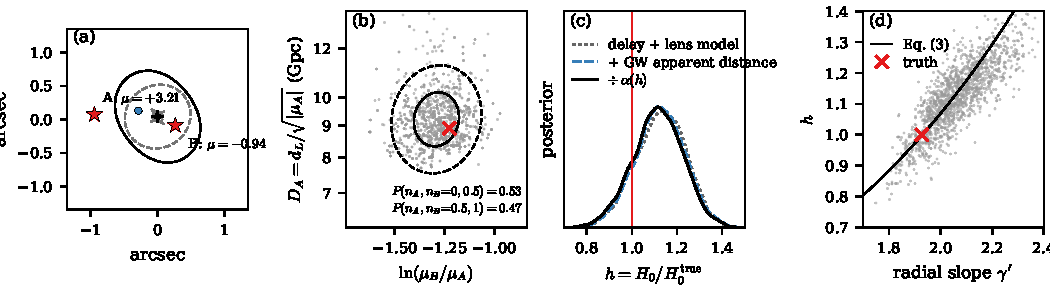
\includegraphics[width=\textwidth]{fig_example.pdf}
\caption{One ET system of the EPL+shear family. (a) Image plane: the two GW images (stars) with their magnifications, the lens center ($+$), the critical curve (solid), the caustic (dashed) and the source position (dot); $z_l=0.81$, $z_s=2.01$, $\theta_E=0.64$\,arcsec, $\gamma'=1.93$, $\Delta t=68.2$\,days. (b) Joint-PE posterior of the magnification ratio and the apparent distance of image $A$ (points, weighted to remove the PE priors), the Gaussian summary used as the GW likelihood (1 and 2 standard deviations), the truth ($\times$) and the probabilities of the two most likely Morse-index combinations. (c) Posterior of $h$ from the delay and the lens model alone, with the GW apparent distance, and divided by the selection fraction; the vertical line marks the truth. (d) Joint posterior of the slope and $h$ with the degeneracy direction of Eq.~\eqref{eq:slope} through the posterior medians.}
\label{fig:example}
\end{figure*}

The posterior of $h$ from the delay and the lens model alone has a median of 1.13 and a 90\% interval of 0.94--1.30 [Fig.~\ref{fig:example}(c)]. Adding the GW apparent distance changes it to 1.13 (0.94--1.30), and dividing by the selection fraction of the ET EPL+shear population to 1.12 (0.92--1.29): for ET neither the amplitude nor the selection term matters much for a single system. The posterior is high because the slope is: $\gamma'=2.05\pm0.11$ against the true 1.93, and $h$ follows the slope along the direction of Eq.~\eqref{eq:slope}, with a correlation coefficient of 0.82 between $\gamma'$ and $\ln h$ [Fig.~\ref{fig:example}(d)]. The system illustrates the general result of Sec.~\ref{sec:information}: the width of $h$ (standard deviation 0.11) is the width of the slope prior, narrowed little by the data, and the GW amplitude adds no information that the delay does not already carry. Appendix~\ref{app:example} shows the posteriors of all parameters of this system, from the joint parameter estimation of the GW data and from the GW+EM analysis.

\section{Results}
\label{sec:results}
\subsection{The two corrections}
\label{sec:corrections}
Figure~\ref{fig:corrections} shows the combined posterior of $h$ when every system is analyzed with the EPL+shear model. Without either correction, the combined estimate is $h=1.054\pm0.010$ for ET and $1.118\pm0.019$ for O5, 5 and 6 standard deviations above the truth. Normalizing the source-position prior, Eq.~\eqref{eq:sourceprior}, lowers these to $1.027^{+0.011}_{-0.010}$ and $1.067^{+0.021}_{-0.020}$, and dividing by the selection fraction gives $1.022\pm0.010$ and $1.010^{+0.017}_{-0.015}$. The selection term alone, without the normalization, would leave $1.050^{+0.010}_{-0.012}$ and $1.068^{+0.017}_{-0.021}$; both corrections are needed.

The selection term matters much more for O5 than for ET [Fig.~\ref{fig:corrections}(a)]. ET detects 42--51\% of all lensed systems of our populations, and its selection fraction grows only as $\alpha\propto h^{0.9}$. O5 detects about 1\%, mostly strongly magnified systems near its threshold, and $\alpha\propto h^{2.7\text{--}2.9}$. A system near the O5 threshold is therefore much more likely to have been detected if $H_0$ is large, and each per-system posterior is shifted upward by about $2.8\,\sigma_h^2$, where $\sigma_h$ is its width; the selection term removes this shift. For the models of the simulated families, which have no free slope except for the EPL+shear family, the normalization of the source prior matters less: it moves the combined $h$ from $1.016\pm0.007$ to $1.010\pm0.008$ (ET) and from $0.994^{+0.015}_{-0.012}$ to $1.001\pm0.011$ (O5), with the selection term included in both.

\begin{figure*}
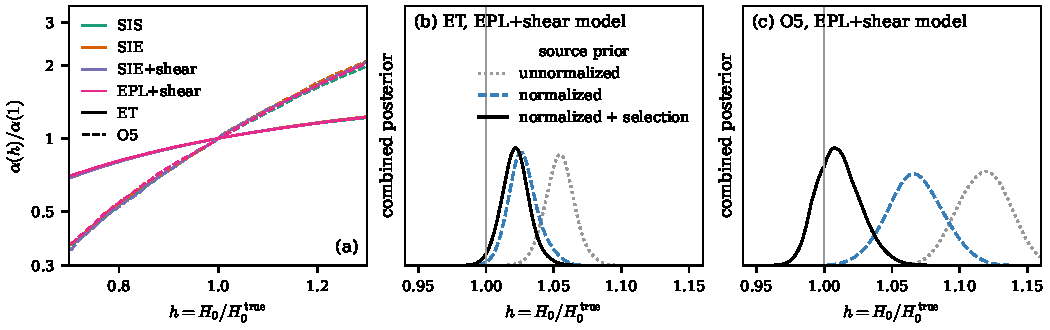
\includegraphics[width=\textwidth]{fig_corrections.pdf}
\caption{(a) Selection fraction $\alpha(h)$ of the four lens populations relative to its value at the true Hubble constant, for ET (solid) and O5 (dashed). (b,c) Combined posterior of $h=H_0/H_0^{\rm true}$ for 60 ET and 59 O5 systems, each analyzed with an EPL+shear lens model: with a source-position prior that is not normalized per lens (dotted), with the normalized prior of Eq.~\eqref{eq:sourceprior} (dashed), and with both the normalized prior and the selection term of Eq.~\eqref{eq:joint} (solid).}
\label{fig:corrections}
\end{figure*}

\subsection{Combined and per-system results}
\label{sec:joint}
Figure~\ref{fig:persystem} shows the posterior of every system with both corrections, and Table~\ref{tab:h0} the combined values; the Supplemental Material~\cite{supplement} lists the true values and posteriors of every system. The combined $h$ is consistent with the truth within 1.4 standard deviations when each system is analyzed with the model of its family ($1.010^{+0.008}_{-0.007}$ for ET, $1.001\pm0.011$ for O5) and within 2.2 standard deviations with the EPL+shear model for every system ($1.022\pm0.010$ and $1.010^{+0.017}_{-0.015}$). The precision of a single system is set by its lens model: the median standard deviation of $h$ is 0.070 for ET and 0.123 for O5 with the model of the family, and 0.103 and 0.151 with the EPL+shear model. The most precise ET systems reach $\sigma_h\approx0.03$, close to the floor of 0.025 set by the prior of $\kappa_{\rm ext}$. The O5 intervals are wider because the O5 systems are the strongly magnified ones (Table~\ref{tab:sample}): their GW images lie close to each other and to the critical curve, where the Fermat-potential difference is small and its fractional uncertainty, for the same lens-model uncertainty, is larger.

The 90\% intervals of individual systems contain the true value for 92\% (ET) and 83\% (O5) of the systems with the model of their family, and for 95\% and 93\% with the EPL+shear model, which gives wider intervals. Appendix~\ref{app:calibration} examines the calibration in detail. The O5 shortfall is confined to strongly magnified systems: when the brighter GW image has $|\mu|<5$, the intervals contain the truth for 95\% of the 22 O5 systems; when $|\mu|\ge5$, for only 76\% of the 37 others. Near a fold caustic the delay between the two merging images, like their magnifications (Paper~I), depends steeply on the source position and the lens model, and the intervals of these systems are too narrow. At the present precision this does not bias the combined value, but it would matter for larger samples. ET detects few such systems (6 of 60, of whose intervals 5 contain the truth).

\begin{table*}
\caption{Combined Hubble constant $h=H_0/H_0^{\rm true}$ (median and 68\% interval) from 60 ET and 59 O5 systems, with the normalized source prior and the selection term; median per-system standard deviation $\sigma_h$; and fraction of per-system 90\% intervals that contain $h=1$ (cov.). Each system is analyzed with the lens model of its simulated family or with an EPL+shear model. In the rows with $\kappa_{\rm ext}$ drawn, the data of each system are rescaled for an external convergence drawn from the prior of the analysis, $\mathcal N(0,0.025)$.}
\label{tab:h0}
\footnotesize
\begin{tabular*}{\linewidth}{@{\extracolsep{\fill}}lcccccc@{}}
\toprule
 & \multicolumn{3}{c}{ET (60 systems)} & \multicolumn{3}{c}{O5 (59 systems)}\\
\cmidrule(lr){2-4}\cmidrule(l){5-7}
Lens model, data & $h$ & $\sigma_h$ & cov. & $h$ & $\sigma_h$ & cov.\\
\midrule
Simulated family, $\kappa_{\rm ext}=0$ & $1.010^{+0.008}_{-0.007}$ & 0.070 & 0.92 & $1.001^{+0.011}_{-0.011}$ & 0.123 & 0.83\\
EPL+shear, $\kappa_{\rm ext}=0$ & $1.022^{+0.010}_{-0.010}$ & 0.103 & 0.95 & $1.010^{+0.017}_{-0.015}$ & 0.151 & 0.93\\
Simulated family, $\kappa_{\rm ext}$ drawn & $1.014^{+0.008}_{-0.008}$ & 0.070 & 0.88 & $0.993^{+0.010}_{-0.009}$ & 0.122 & 0.81\\
EPL+shear, $\kappa_{\rm ext}$ drawn & $1.020^{+0.011}_{-0.011}$ & 0.105 & 0.97 & $0.994^{+0.015}_{-0.012}$ & 0.151 & 0.90\\
\bottomrule
\end{tabular*}

\end{table*}

\subsection{External convergence}
\label{sec:kext}
In the baseline systems the true external convergence is zero, while the analysis allows $\kappa_{\rm ext}\sim\mathcal N(0,0.025)$. To test the treatment of the mass sheet, we rescaled the data of each system as for an external convergence drawn from this prior: the image positions and the magnification ratio are unchanged, the magnifications scale as $(1-\kappa_{\rm ext})^{-2}$, and the apparent distance and the delay as $1-\kappa_{\rm ext}$; the velocity dispersion, which the lens model relates to the Einstein radius without the sheet, is unchanged. The combined $h$ remains consistent with the truth, $1.014\pm0.008$ (ET) and $0.993^{+0.010}_{-0.009}$ (O5) with the model of the family and $1.020\pm0.011$ and $0.994^{+0.015}_{-0.012}$ with the EPL+shear model, and the per-system widths are essentially unchanged (Table~\ref{tab:h0}). This test assumes that the prior describes the line-of-sight population correctly. By Eqs.~\eqref{eq:dt} and \eqref{eq:da}, a mean external convergence that differs from the mean of the prior by $\delta\bar\kappa$ shifts the combined $h$ by $-\delta\bar\kappa$, and this offset does not decrease with the number of systems.

\begin{figure*}
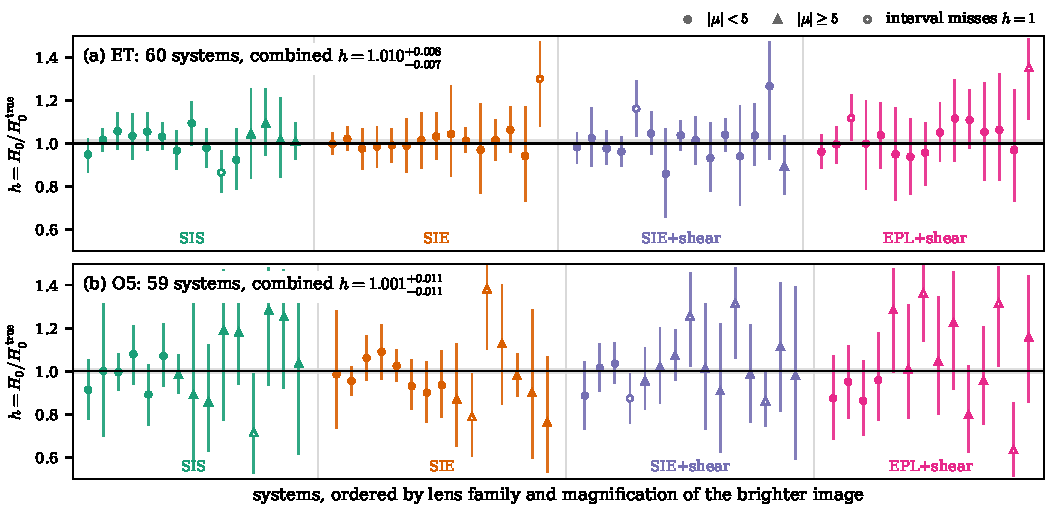
\includegraphics[width=\textwidth]{fig_persystem.pdf}
\caption{Posterior of $h$ for each system (median and 90\% interval, with the normalized source prior and the selection term), analyzed with the lens model of its simulated family, for (a) ET and (b) O5. Within each family the systems are ordered by the magnification of the brighter GW image; triangles mark $|\mu|\ge5$, open symbols intervals that do not contain the truth. The gray band is the 68\% interval of the combined posterior.}
\label{fig:persystem}
\end{figure*}

\subsection{Where the information comes from}
\label{sec:information}
Figure~\ref{fig:delay} compares the per-system width of $h$ with and without the GW apparent distance in the likelihood. Without it, $h$ is determined by the delay and the lens model alone, as in time-delay cosmography. The per-system standard deviations increase by a median of 4\% (ET) and 3\% (O5), with 10--90\% ranges of $-3$ to $+26\%$ and $-2$ to $+19\%$, and the medians move by 0.16 and 0.15 standard deviations. Combining all systems with inverse-variance weights, the width increases by 4\% for ET and 2\% for O5. The GW amplitude therefore adds little: the information on $H_0$ comes from the millisecond delay combined with the lens model. The apparent distance constrains $h$ only together with the absolute magnification predicted by the same lens model, whose uncertainty is set by the same parameters that limit the delay prediction, and it is measured only to $\sigma_{\ln D}\approx0.1$ even by joint parameter estimation of ET data (Paper~I).

\begin{figure}
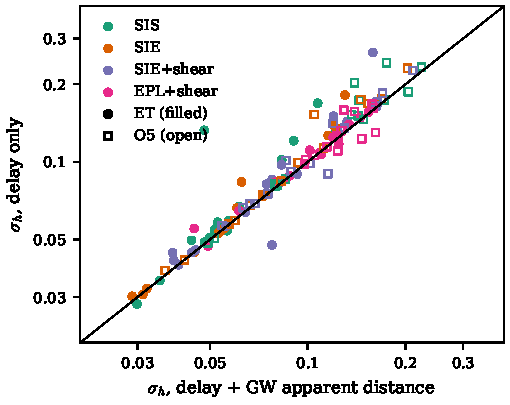
\includegraphics[width=\columnwidth]{fig_delay.pdf}
\caption{Per-system standard deviation of $h$ from the delay and the lens model alone versus that with the GW apparent distance included, for ET (filled) and O5 (open) systems analyzed with the model of their family. The line marks equal widths.}
\label{fig:delay}
\end{figure}

The accuracy is therefore limited, as in time-delay cosmography with lensed quasars, by the lens model, and above all by the radial slope, Eq.~\eqref{eq:slope}. Figure~\ref{fig:slope} shows the offset of the combined $h$ for each lens family. With the model of the family the offsets are within 1.6 standard deviations of zero. With the EPL+shear model, the slopes of the isothermal SIS and SIE lenses ($\gamma'=2$) are pulled toward the prior mean of 2.08, because two images with a measured magnification ratio constrain the slope only weakly. For ET the posterior median of the slope exceeds the true value by $0.047\pm0.016$ (SIS) and $0.039\pm0.015$ (SIE) on average, which by Eq.~\eqref{eq:slope} raises $h$ by $4.7\pm1.6\%$ and $3.9\pm1.5\%$; the measured offsets are $4.8\pm2.6\%$ and $2.4\pm2.2\%$. For the EPL+shear family, analyzed with the prior from which its slopes were drawn, the mean slope error is $+0.044\pm0.019$ and the offset $2.8\pm2.1\%$; with 15 systems we cannot tell whether this is a residual bias or a fluctuation. The excess of the ET combination with the EPL+shear model, $2.2\pm1.0\%$, is of the size expected from these slope errors. For O5 the per-family offsets are consistent with zero within their larger uncertainties.

\begin{figure*}
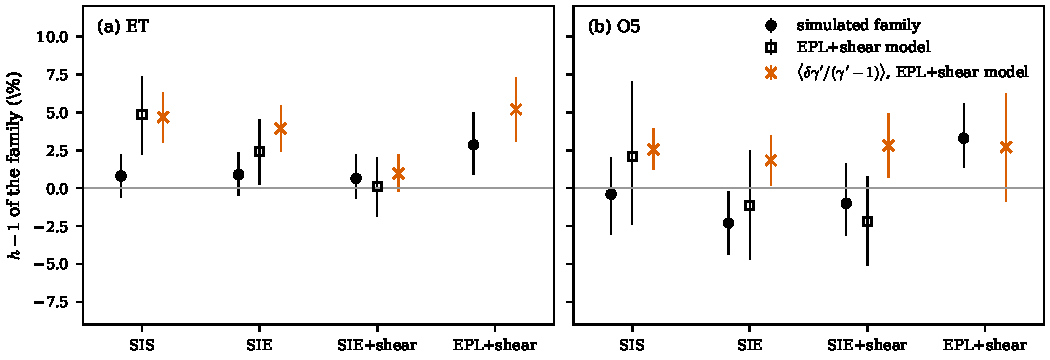
\includegraphics[width=\textwidth]{fig_slope.pdf}
\caption{Offset of the combined $h$ for each lens family (15 systems; 14 for O5 EPL+shear), analyzed with the model of the family (filled circles) or with an EPL+shear model (open squares; for the EPL+shear family the two coincide). Crosses: mean of $\delta\gamma'/(\gamma'-1)$ over the systems of the family analyzed with the EPL+shear model, where $\delta\gamma'$ is the difference between the posterior median and the true slope, i.e. the offset expected from the slope error by Eq.~\eqref{eq:slope}. Error bars are 68\% intervals and standard errors of the mean.}
\label{fig:slope}
\end{figure*}

\section{Discussion}
\label{sec:discussion}
\subsection{Implications for real data}
The two corrections apply to any population analysis of lensed GWs with identified hosts. The source-position prior and the lens prior must together reproduce the joint distribution of lens and source parameters of the population from which the systems come (Sec.~\ref{sec:sourceprior}). In real data this means that a flat source prior should be combined with the intrinsic distribution of lens parameters, or a prior derived from observed lenses with a source prior normalized per lens. The selection fraction $\alpha(h)$ must be computed from a model of the detection of both GW images and, unlike here, of the identification of the host and the lens in EM data; for networks that detect only the most magnified systems, it is not a small correction.

Our results also show what limits the accuracy. The lens prior, in particular that of the slope, must describe the population of lenses from which the detected systems are drawn, before selection; the selection is then accounted for by $\alpha(h)$. A mean offset $\delta\bar\gamma'$ between the prior and that population biases $H_0$ by about $\delta\bar\gamma'/(\gamma'-1)$, and a mean offset $\delta\bar\kappa$ of the external convergence by $-\delta\bar\kappa$; neither decreases with the number of systems. Detected lenses are not representative of their parent population, because detection favors highly magnified images: in our simulations the mean slope of detected EPL+shear lenses is 2.01 for ET and 1.93 for O5, compared with 2.08 for the parent population [Fig.~\ref{fig:sample}(d)], and lensed quasars show the same effect \citep{collett2016selection,li2024selection}. The slope distribution could be inferred jointly with $H_0$ from the population of systems, as in time-delay cosmography with lensed quasars \citep{birrer2020tdcosmo,tdcosmo2025}, and the radial profile of each lens could be constrained by stellar kinematics interpreted with a dynamical model or by extended arcs of the lensed host. The external convergence requires line-of-sight estimates from galaxy counts or ray tracing for each system \citep{rusu2017kext}.

With these provisos, the precision scales as $\sigma_h\approx0.07/\sqrt N$ for $N$ ET systems like ours and $0.12/\sqrt N$ for O5, so that a 2\% measurement requires about 12 ET or 36 O5 systems, provided that the slope and external-convergence priors are accurate to well below 2\%. The per-system precision is several times that assumed in the forecast of Ref.~\citep{liao2017precision}, about 1.2\%, because our EM data, two image positions, the lens light and the velocity dispersion, leave the slope close to its prior width. An uncertainty of 0.6\% in the Fermat-potential difference corresponds by Eq.~\eqref{eq:slope} to a slope measured to about 0.006 for each system, which requires modeling of the extended images of the lensed host \citep{hannuksela2020localizing,wempe2022lensing}. At that precision the two corrections matter even more, because the biases they remove, 5\% to 12\% here, do not decrease with the number of systems.

\subsection{Limitations}
\label{sec:limitations}
We assumed, as in Paper~I, that the GW images have been associated with each other and with an identified host, and that the image positions of the BBH within the host have been reconstructed to 0.01\,arcsec; this reconstruction is a separate inference that we have not simulated. The lens families are idealized: they contain no satellites or line-of-sight structures beyond a uniform external convergence, and the velocity dispersion only sets the Einstein radius. The GW data are Gaussian noise with aligned spins. The selection fraction is computed with the same detection model as the simulation, so the test does not include errors in modeling the selection. With 15 systems per family and scenario, biases are tested at the level of 1--2\% for the combined samples and 2--5\% per family. Finally, the per-system intervals of strongly magnified systems are too narrow (Sec.~\ref{sec:joint} and Appendix~\ref{app:calibration}).

\section{Conclusions}
\label{sec:conclusions}
We have tested Hubble-constant inference from strongly lensed BBHs with identified host galaxies, using 60 ET and 59 O5 systems from four lens families, joint parameter estimation of both GW images from simulated detector data and a Bayesian reconstruction of the lens.
\begin{enumerate}
\item Two corrections are required. The source-position prior must be normalized for each lens as in the population from which the systems come, and the selection fraction $\alpha(H_0)$ of detectable systems must divide the likelihood. Without them, an EPL+shear analysis overestimates $H_0$ by 5\% (ET) and 12\% (O5).
\item With both corrections the combined estimate is consistent with the truth: $H_0/H_0^{\rm true}=1.010^{+0.008}_{-0.007}$ (ET) and $1.001\pm0.011$ (O5) with the models of the simulated families and $1.022\pm0.010$ and $1.010^{+0.017}_{-0.015}$ with an EPL+shear model for every system, also when an external convergence is drawn for each system. A single system constrains $H_0$ to a median 7\% (ET) and 12\% (O5).
\item The information comes from the delay and the lens model. The GW apparent distance narrows the per-system intervals by only 3--4\%. The accuracy is therefore limited by the priors on the radial slope and the external convergence: a slope prior that does not describe the lenses biases a family by up to 5\%, and the prior must describe the lenses before selection, whose mean slope differs from that of the detected lenses by 0.07 (ET) and 0.15 (O5) in our simulations.
\item The per-system intervals of strongly magnified systems ($|\mu|\ge5$) contain the truth too rarely, which matters for O5, where most detected systems are strongly magnified.
\end{enumerate}
